%%%%%%%%%%%%%%%%%%%%%%%%%%%%%%%%%%%%%%%%%
% Beamer Presentation
% LaTeX Template
% Version 1.0 (10/11/12)
%
% This template has been downloaded from:
% http://www.LaTeXTemplates.com
%
% License:
% CC BY-NC-SA 3.0 (http://creativecommons.org/licenses/by-nc-sa/3.0/)
%
%%%%%%%%%%%%%%%%%%%%%%%%%%%%%%%%%%%%%%%%%

%----------------------------------------------------------------------------------------
%	PACKAGES AND THEMES
%----------------------------------------------------------------------------------------

\documentclass{beamer}

\mode<presentation> {

% The Beamer class comes with a number of default slide themes
% which change the colors and layouts of slides. Below this is a list
% of all the themes, uncomment each in turn to see what they look like.

\usetheme{default}
%\usetheme{AnnArbor}
%\usetheme{Antibes}
%\usetheme{Bergen}
%\usetheme{Berkeley}
%\usetheme{Berlin}
%\usetheme{Boadilla}
%\usetheme{CambridgeUS}
%\usetheme{Copenhagen}
%\usetheme{Darmstadt}
%\usetheme{Dresden}
%\usetheme{Frankfurt}
%\usetheme{Goettingen}
%\usetheme{Hannover}
%\usetheme{Ilmenau}
%\usetheme{JuanLesPins}
%\usetheme{Luebeck}
%\usetheme{Madrid}
%\usetheme{Malmoe}
%\usetheme{Marburg}
%\usetheme{Montpellier}
%\usetheme{PaloAlto}
%\usetheme{Pittsburgh}
%\usetheme{Rochester}
%\usetheme{Singapore}
%\usetheme{Szeged}
%\usetheme{Warsaw}

% As well as themes, the Beamer class has a number of color themes
% for any slide theme. Uncomment each of these in turn to see how it
% changes the colors of your current slide theme.

%\usecolortheme{albatross}
%\usecolortheme{beaver}
%\usecolortheme{beetle}
%\usecolortheme{crane}
%\usecolortheme{dolphin}
%\usecolortheme{dove}
%\usecolortheme{fly}
%\usecolortheme{lily}
%\usecolortheme{orchid}
%\usecolortheme{rose}
%\usecolortheme{seagull}
%\usecolortheme{seahorse}
%\usecolortheme{whale}
%\usecolortheme{wolverine}

%\setbeamertemplate{footline} % To remove the footer line in all slides uncomment this line
%\setbeamertemplate{footline}[page number] % To replace the footer line in all slides with a simple slide count uncomment this line

%\setbeamertemplate{navigation symbols}{} % To remove the navigation symbols from the bottom of all slides uncomment this line
}

\usepackage{graphicx} % Allows including images
\usepackage{booktabs} % Allows the use of \toprule, \midrule and \bottomrule in tables
\usepackage{url}
\usepackage[T1]{fontenc}
\usepackage[utf8]{inputenc}


%----------------------------------------------------------------------------------------
%	TITLE PAGE
%----------------------------------------------------------------------------------------

\title[Lab 5]{Lab 5: Cubic Splines} % The short title appears at the bottom of every slide, the full title is only on the title page

\author{Kasper Høj Lorenzen} % Your name
\institute[SDU Robotics] % Your institution as it will appear on the bottom of every slide, may be shorthand to save space
{
Univeristy of Southern Denmark \\ % Your institution for the title page
\medskip
\textit{kalor@mmmi.sdu.dk} % Your email address
}
\date{October 6, 2022} % Date, can be changed to a custom date

\begin{document}

\begin{frame}
\titlepage % Print the title page as the first slide
\end{frame}

\begin{frame}
\frametitle{Overview} % Table of contents slide, comment this block out to remove it
\tableofcontents % Throughout your presentation, if you choose to use \section{} and \subsection{} commands, these will automatically be printed on this slide as an overview of your presentation
\end{frame}

%----------------------------------------------------------------------------------------
%	PRESENTATION SLIDES
%----------------------------------------------------------------------------------------

% ------------------------------------------------

\section{Programming Exercise 5.1}

% ------------------------------------------------

\begin{frame}
  \frametitle{Cubic Splines}
  \begin{itemize}
  \item Interpolate between two poitns
  \item Path goes through the two points
    \begin{itemize}
      \item In contrast to Parabolic blends
    \end{itemize}
  \item Each point can be specified with a velocity and/or time
  \item Cubic splines interpolate postions, velocities and accelerations to satisfy constraints
  \item Position, velocity and acceleration are contiuous
  \end{itemize}
\end{frame}

% ------------------------------------------------

\begin{frame}
  \frametitle{Cubic Splines}
  \begin{itemize}
  \item Implement this function and test it on a 2D path
  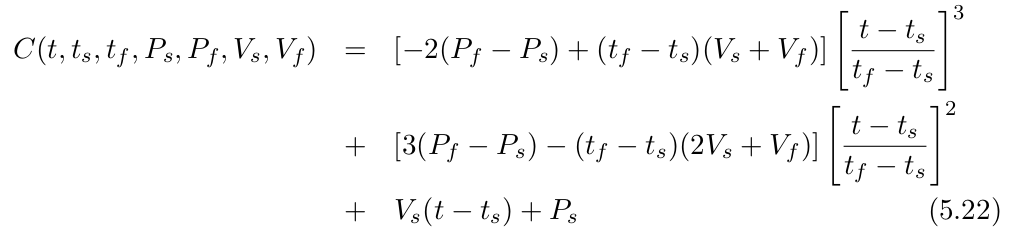
\includegraphics[width=\textwidth]{./cubic_spline_equation}
  \end{itemize}
\end{frame}

% ------------------------------------------------

\begin{frame}
  \frametitle{Programming Exercise 5.1}
  \begin{columns}
    \begin{column}{0.6\textwidth}
      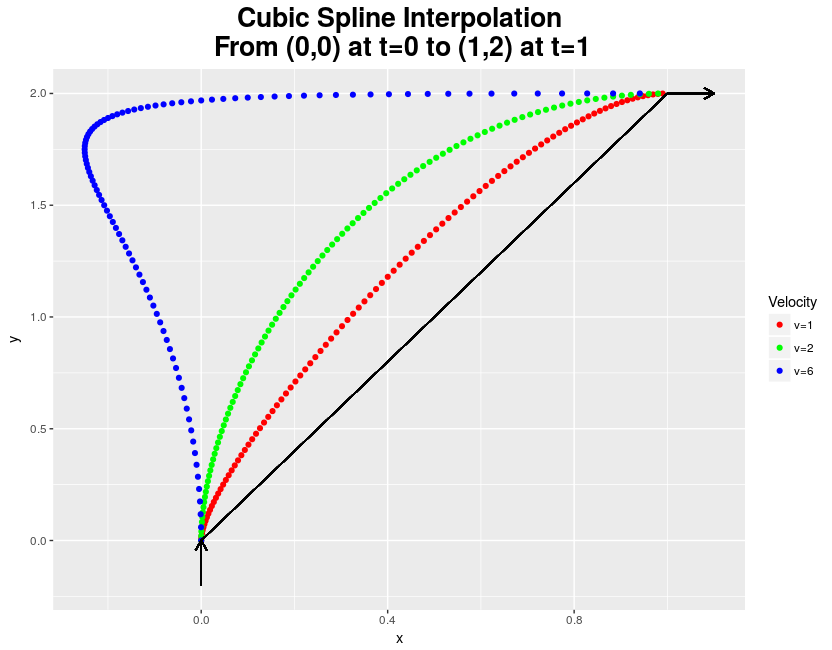
\includegraphics[width=\textwidth]{./cubic_spline}
    \end{column}
    \begin{column}{0.4\textwidth}
      \begin{itemize}
      \item Arrows show the direction of velocities at the start and end points
      \item Linear interpolation shown as reference (black line)
      \item Velocities:
        \begin{itemize}
          \item Red - $(0,1) \rightarrow (1,0)$
          \item Green - $(0,2) \rightarrow (2,0)$
          \item Blue - $(0,6) \rightarrow (6,0)$
        \end{itemize}
      \end{itemize}
    \end{column}
  \end{columns}
\end{frame}

% ------------------------------------------------
%----------------------------------------------------------------------------------------

\end{document} 
